\section{Why Leak-Free Scores Are Low}
\label{sec:why}

\subsection{The Annotators Against Themselves}
WTBD's augmented copies were annotated independently, so aligned copies of an image give accidental repeated labels. For every verified pair of the same surface we project each label through the estimated transform. The transform is a flip-aware ORB + RANSAC similarity with at least 25 inliers, and at least 8 of them inside the box. We then classify the label as \emph{agree} (same class, IoU~$\geq0.5$), \emph{class conflict}, \emph{split}, \emph{loose} or \emph{missing}. Fig.~\ref{fig:ambiguity} shows examples, and Table~\ref{tab:selfconsistency} gives the rates.

\begin{figure*}[!t]
\centering
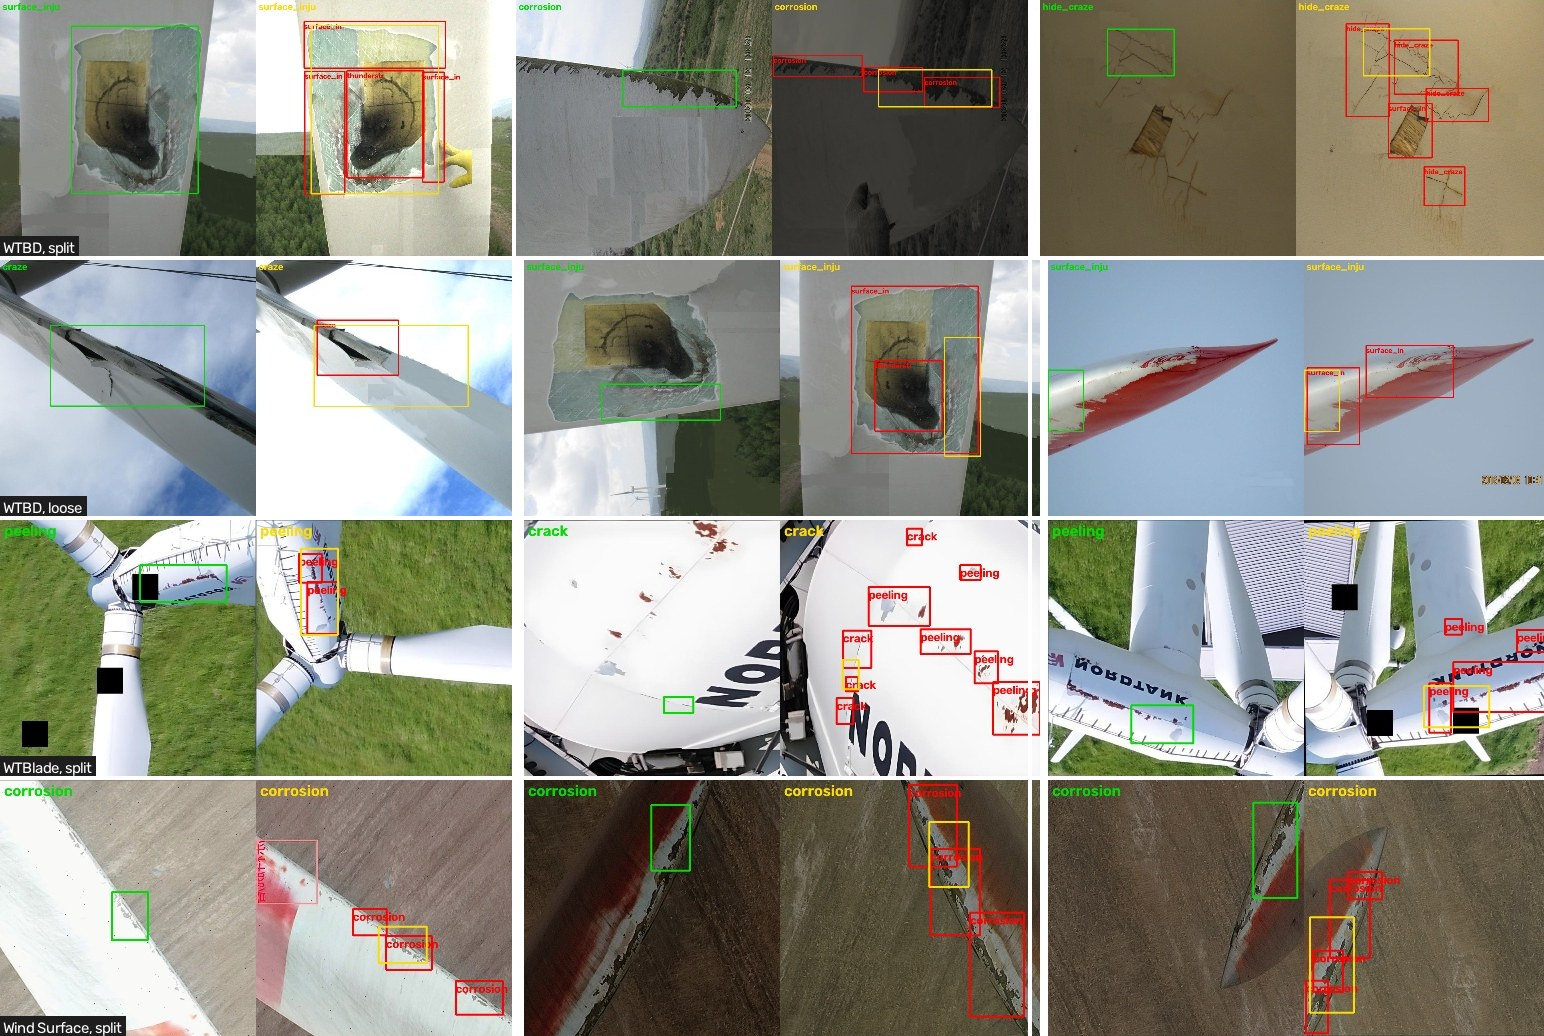
\includegraphics[width=0.86\textwidth]{fig11_label_ambiguity}
\caption{Annotation ambiguity on aligned copies. In each pair, left: a label (green); right: its exact projection (yellow) and what the copy's annotator drew (red). Top two rows: WTBD. Third row: WTBlade-Defect. Bottom row: Wind Surface. The disagreement is about extent and about how a defect is cut into boxes, not about the class. ``NORDTANK'' is legible in the third row.}
\label{fig:ambiguity}
\end{figure*}

\begin{table}[!t]
\centering
\caption{Label self-consistency on axis-aligned copies of the same image (rotation within 3$^\circ$ of a multiple of 90$^\circ$, flips included), where boxes map to boxes and every difference is an annotation difference. Rotated copies and other views agree less, but those strata also include geometric effects.}
\label{tab:selfconsistency}
\footnotesize
\setlength{\tabcolsep}{2.2pt}
\begin{tabular}{@{}l r r r r r r r r@{}}
\toprule
Dataset & Labels & Agree & Split & Loose & Miss & Class & Rot. & Other \\
\midrule
WTBD & 2{,}965 & \textbf{87.3} & 4.6 & 6.7 & 1.5 & 0 & 77.9 & 64.1 \\
WTBlade & 42{,}812 & \textbf{86.0} & 2.5 & 8.2 & 3.1 & 91 & 80.7 & 59.8 \\
Wind Surf. & 10{,}261 & \textbf{83.8} & 9.2 & 5.9 & 1.1 & 0 & (18) & 44.2 \\
\bottomrule
\end{tabular}
\tabnote{Percent of labels, except \emph{Class}: number of class conflicts (0.2\% on WTBlade). \emph{Rot.}: agreement on rotated copies; \emph{Other}: on other views of the surface.}
\end{table}

So 13--16\% of labels disagree with an exactly aligned copy in all three datasets, including one that was double-annotated ($\kappa=0.897$~\cite{wtbd}). Almost none of the disagreement is about class. The amorphous classes are the least consistent (Fig.~\ref{fig:agreement}). Counts are per label occurrence, and they concentrate in a few heavily duplicated scenes. On WTBlade the ``missing'' rate is mostly a matching artefact of rotating rotors in video (1.1\% without dirt). Most of its 91 class conflicts are pasted synthetic patches, labelled peeling in one copy and crack in another.

\begin{figure}[!t]
\centering
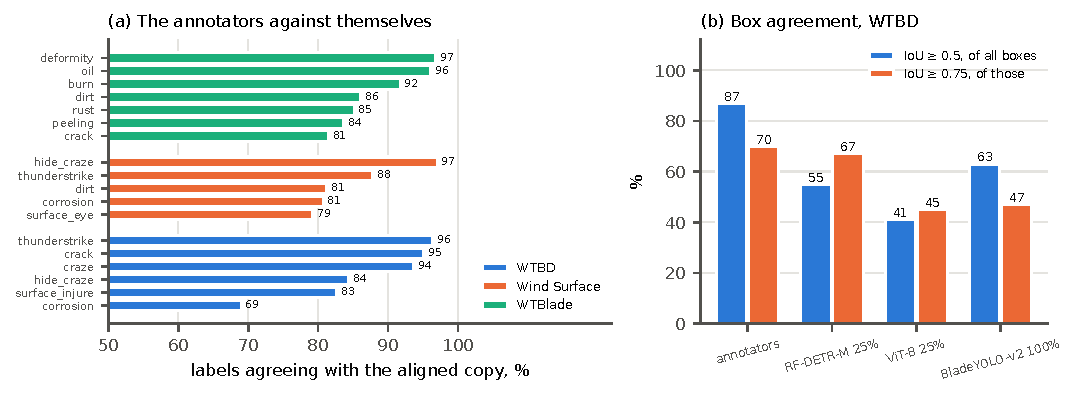
\includegraphics[width=\linewidth]{fig12_label_agreement}
\caption{(a) Per-class agreement on aligned copies. (b) Box agreement on WTBD: how often an independent annotator's box, or a detector's best box, reaches IoU 0.5, and of those, how many reach 0.75 (confidence $\geq$0.1 for detectors). RF-DETR-M at 25\% labels matches the annotators on extent once it finds a defect (0.67 against 0.70; median IoU 0.83 for both).}
\label{fig:agreement}
\end{figure}

\subsection{Box Granularity}
On WTBD-group, tolerant \apfifty exceeds standard \apfifty by $+11.9$ for BladeYOLO-v2 (56.1 to 68.0) and by $+12.4$ for YOLO12-L (40.0 to 52.4). The most striking class is craze, which rises from 9.9 to 66.1. All 15 craze test images are rotated, flipped or recoloured copies of one long leading-edge split, annotated as 2--3 segment boxes (Fig.~\ref{fig:craze}). The same effect holds for RF-DETR scored with classes merged: \apfifty rises from 66.1 to 79.7 on WTBD-group and from 50.1 to 61.2 on WTBlade-group. Table~\ref{tab:granularity} gives the per-class view.

\begin{figure}[!t]
\centering
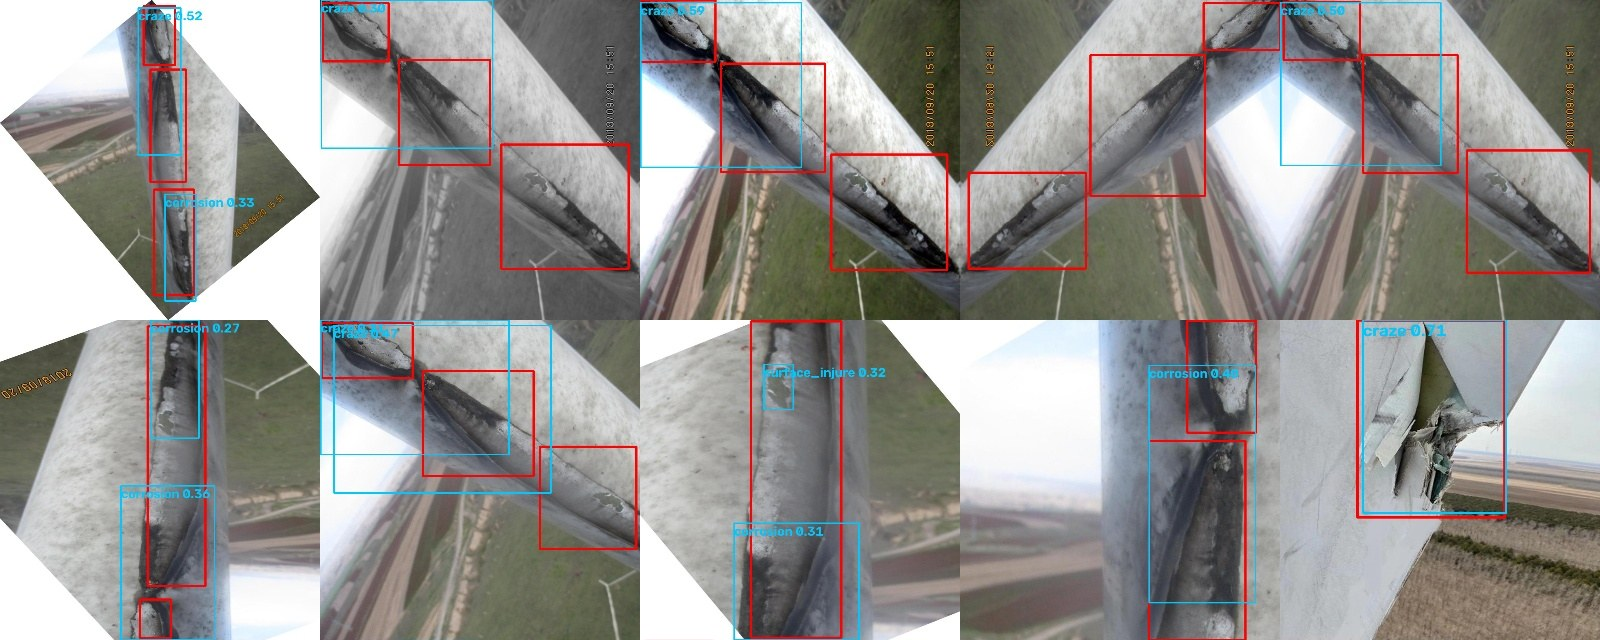
\includegraphics[width=\linewidth]{fig13_craze_scene}
\caption{All 15 WTBD-group craze test images come from one scene. Red: labels, split into segments by the annotator. Blue: BladeYOLO-v2 predictions. The model often draws one box where the label has several, which counts as an error at IoU 0.5 and explains most of the ``craze failure''.}
\label{fig:craze}
\end{figure}

\begin{table}[!t]
\centering
\caption{Three box scores on WTBD-group test, in percent (500 scene replicates). Per class: BladeYOLO-v2. The official-minus-group gap shrinks as the metric becomes split-invariant (BladeYOLO-v2: $+25.4$, $+20.9$, $+16.8$). \best{Red bold}: better model on each split.}
\label{tab:granularity}
\scriptsize
\setlength{\tabcolsep}{1.5pt}
\begin{tabularx}{\linewidth}{@{}X l l l@{}}
\toprule
& Std.\ \apfifty & Tol.\ \apfifty & Region AP \\
\midrule
BYv2, group & \best{56.1} \ci{48.3}{79.1} & \best{68.0} \ci{60.4}{83.1} & \best{60.3} \ci{55.2}{74.3} \\
YOLO12-L, group & 40.0 \ci{33.9}{67.8} & 52.4 \ci{46.5}{74.0} & 44.1 \ci{40.2}{59.2} \\
difference & $+16.1$ \ci{+2.3}{+28.4} & $+15.6$ \ci{+0.1}{+23.7} & $\mathbf{+16.2}$ \ci{+7.7}{+23.6} \\
BYv2, official & \best{81.5} & \best{88.9} & \best{77.1} \\
YOLO12-L, official & 69.0 & 80.0 & 66.6 \\
\midrule
craze & 9.9 & \textbf{66.1} & 42.7 \\
corrosion & 62.6 & 67.6 & 68.4 \\
surface\_injure & 75.9 & 81.6 & 68.9 \\
thunderstrike & 100.0 & 100.0 & 68.2 \\
crack & 35.2 & 35.6 & 49.1 \\
hide\_craze & 53.0 & 56.8 & 64.5 \\
\bottomrule
\end{tabularx}
\end{table}

Two limits apply. First, we hypothesised that part of the leakage inflation is memorised box splitting, and tested it. The tolerant gain is not smaller on test images with a training twin, so the hypothesis is not supported. Second, training a detector to tolerate splitting does not help overall. Blanket split-tolerant training is not an improvement (tolerant \apfifty $+1.5$ \ci{-11.1}{+6.4}). Class-selective tolerance raises corrosion by $+9.3$ \ci{-0.3}{+24.6}, while the mean moves by $-0.4$. The ambiguity therefore limits what can be measured more than what can be trained away.

\textbf{Annotators as a ceiling.} Corrosion copies agree on only 69\% of labels, and models score near that (BladeYOLO-v2 \apfifty 54--63), so further corrosion ``improvement'' is largely unmeasurable with these labels. Crack copies agree on 95\% while the YOLO family scores 35--39, so crack is a genuine model weakness there.

\subsection{Subset Luck}
At a fixed budget of 25\% of scenes, which scenes are labelled matters more than any model effect we measured (Fig.~\ref{fig:luck}). Across 8 random draws with the same model, recipe and seed, ViT-B test \mcoco spans 9.0--19.6 ($\times2.2$); without DINOv3 it spans 2.6--7.2. The DINOv3 gain holds on 8 of 8 draws ($+7.1$ \ci{+5.1}{+12.6}), and draw quality carries over between models (Spearman $\rho=0.71$). Yet no label-free subset property we tested predicts it (H7, G16, H20). Label-free scene selection by patch coverage beats random by $+5.2$ \ci{+1.9}{+10.5}. It does not separate from FreeSel~\cite{freesel}, however: $+2.1$ \ci{-1.2}{+9.1}, $P=0.917$, with validation pointing the other way. Table~\ref{tab:selection} gives the selection runs at the 25\% budget. Selecting by class balance does worst of the five arms, which suggests that \emph{which} scenes are labelled matters more than matching class counts.

\begin{table}[!t]
\centering
\caption{Selection of which 25\% of WTBD-group scenes to label: 18 ViT-B runs at the same budget, training seed 0. Random draws per run: 11.2, 13.5, 11.8, 12.3, 9.0, 10.0, 12.4, 19.6. \hlnote{}}
\label{tab:selection}
\footnotesize
\setlength{\tabcolsep}{2.4pt}
\begin{tabularx}{\linewidth}{@{}X r r r l@{}}
\toprule
Arm (runs) & Test \mfifty & Test \mcoco & Val \mcoco & Rank (test/val) \\
\midrule
Patch coverage, label-free (4) & \second{40.6} & \best{17.7} & 23.6 & 2/9, 3/9 \\
FreeSel-224 (2) & \best{42.9} & \second{15.6} & \best{27.1} & 2/9, 1/9 \\
FreeSel-640 (2) & 34.4 & 14.5 & \second{26.6} & 2/9, 2/9 \\
Random (8) & 31.3 & 12.5 & 21.6 & \\
Class-matched, uses labels (2) & 25.3 & 10.4 & 19.7 & 7/9, 7/9 \\
\bottomrule
\end{tabularx}
\end{table}

\begin{figure}[!t]
\centering
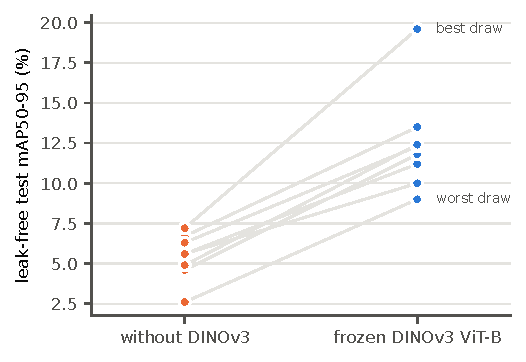
\includegraphics[width=0.9\linewidth]{fig5_subset_luck}
\caption{Subset luck: test \mcoco across random 25\% scene draws, same model, recipe and seed.}
\label{fig:luck}
\end{figure}

\subsection{Error Anatomy}
\label{sec:anatomy}
Scarce labels fail differently by detector family (Fig.~\ref{fig:anatomy}, in the style of TIDE~\cite{tide}). For each test box we ask whether a same-class box at IoU~$\geq0.5$ is among the outputs, and how it is scored. Table~\ref{tab:anatomy} gives the numbers, and Table~\ref{tab:ceiling} the extent comparison.

\begin{figure}[!t]
\centering
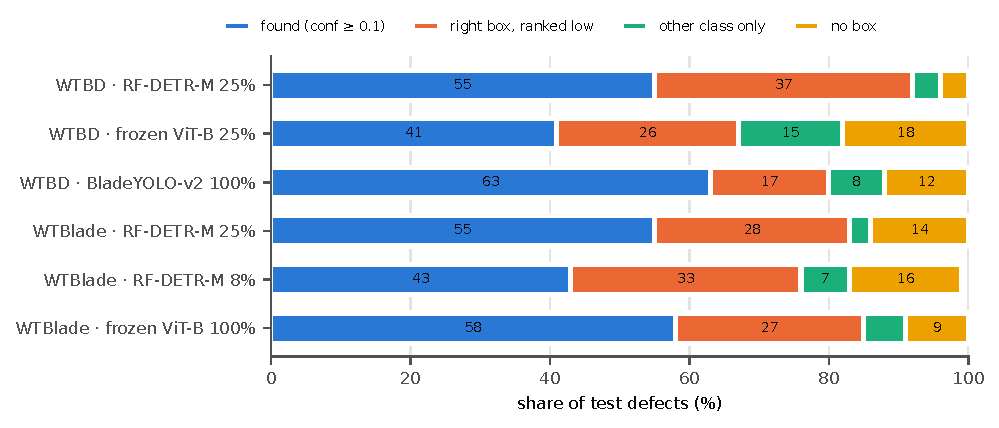
\includegraphics[width=\linewidth]{fig6_error_anatomy}
\caption{Error anatomy. Hit: a same-class box at IoU $\geq$0.5 with confidence $\geq$0.1. Ranked low: such a box exists only below 0.1. Other class: only other-class boxes at IoU $\geq$0.5. No box: nothing at IoU $\geq$0.5.}
\label{fig:anatomy}
\end{figure}

\begin{table}[!t]
\centering
\caption{Error anatomy as a share of test boxes. Candidate recall = hit + ranked low. YOLO-family runs keep fewer boxes after NMS (about 50--80 per image) than RF-DETR (300), so recall within each image's top 50 boxes is also given. \hlnote{} (within each dataset; for Other and None lower is better)}
\label{tab:anatomy}
\footnotesize
\setlength{\tabcolsep}{2pt}
\begin{tabularx}{\linewidth}{@{}X r r r r r r@{}}
\toprule
Detector & Hit & Low & Other & None & Cand. & Top 50 \\
\midrule
\multicolumn{7}{@{}l}{\textit{WTBD-group}} \\
RF-DETR-M 25\% (4 subsets) & \second{0.55} & 0.37 & \best{0.04} & \best{0.04} & \best{0.92} & \best{0.81} \\
ViT-B 25\% (4 subsets) & 0.41 & 0.26 & 0.15 & 0.18 & 0.67 & 0.66 \\
BladeYOLO-v2 100\% (2 seeds) & \best{0.63} & 0.17 & \second{0.08} & \second{0.12} & \second{0.80} & \second{0.80} \\
\multicolumn{7}{@{}l}{\textit{WTBlade-group}} \\
RF-DETR-M 25\% (4 subsets) & \second{0.55} & 0.28 & \best{0.03} & \second{0.14} & \second{0.83} & \second{0.72} \\
RF-DETR-M 8\% (4 subsets) & 0.43 & 0.33 & 0.07 & 0.16 & 0.77 & 0.62 \\
ViT-B 100\% & \best{0.58} & 0.27 & \second{0.06} & \best{0.09} & \best{0.85} & \best{0.81} \\
\bottomrule
\end{tabularx}
\end{table}

\begin{table}[!t]
\centering
\caption{Box extent against the annotator ceiling on WTBD: the same-class IoU of a label with its copy, or of the best prediction with confidence $\geq0.1$, per test box. \hlnote{} (among detectors; annotators are the reference)}
\label{tab:ceiling}
\footnotesize
\setlength{\tabcolsep}{2.2pt}
\begin{tabularx}{\linewidth}{@{}X r r r r r@{}}
\toprule
Source & Boxes & $\geq$0.5 & of those $\geq$0.75 & median & $\geq$0.75 \\
\midrule
Annotators, all copies & 2{,}965 & 0.87 & 0.70 & 0.83 & 0.61 \\
Annotators, test copies & 392 & 0.91 & 0.75 & 0.84 & 0.68 \\
RF-DETR-M 25\% & 940 & \second{0.55} & \best{0.67} & \best{0.83} & \best{0.37} \\
ViT-B 25\% & 940 & 0.41 & 0.45 & 0.73 & 0.19 \\
BladeYOLO-v2 100\% & 235 & \best{0.63} & \second{0.47} & \second{0.74} & \second{0.29} \\
\bottomrule
\end{tabularx}
\end{table}

\begin{itemize}
\item \textbf{RF-DETR at 25\% labels proposes the right box for most defects.} Candidate recall is 0.92 on WTBD, above BladeYOLO-v2 at 100\% (0.80), and 0.83 on WTBlade. Its deficit is scoring: 37\% of WTBD test defects have a correct box scored below 0.1. Once it finds a defect, its box matches the label as well as a second annotator's does.
\item \textbf{On WTBD the rare classes are confused.} Crack is missed or mislabelled, and thunderstrike is found under other classes (54\% located as another class, over 4 subsets). On WTBlade, 43--49\% of crack boxes lack a same-class box at IoU~$\geq0.5$ at every budget (RF-DETR 8\%: 0.47; 25\%: 0.49; ViT-B 100\%: 0.43), so this is not a label-budget problem. Misses concentrate on small boxes (1.00 below 16\,px, 0.65 below 32\,px, 0.22 above 64\,px). Among near-misses, the largest share is shifted boxes (44\%), not split ones.
\item \textbf{Not resolution, on WTBD.} Median defect short sides at 640\,px are 62--148\,px by class.
\end{itemize}
